\section*{Materials and Methods}

\subsection*{Materials and DNA extraction}
We included one individual from each of 94 open-pollinated landrace maize accessions from high and low elevation sites in Mexico and South America (Table S1).  Accessions were provided by USDA germplasm repository or kindly donated by Major Goodman (NCState).  
Sampling locations are shown in Figure~\ref{map}A (see also supp table S1).  
%shouldn't we put table refs in case these change?
Landraces sampled from altitudes $<$1,700 m were considered lowland, while accessions from $>$1,700 m were considered highland (supp table S1).  
%Please fill in information in table S1 from Matt's excel file (dropbox).  
Seeds were germinated on filter paper following fungicide treatment and grown in standard potting mix.  Leaf tips were harvested from plants at the five leaf stage.  Following storage at $-80{}^\circ$C overnight, leaf tips were lyophilized for 48 hours.  Tissue was then homogenized with a Mini-Beadbeater-8 (BioSpec Products, Inc., Bartlesville, OK, USA).  DNA was extracted using a modified CTAB protocol \cite[]{CTAB}.  The quality of DNA was ensured using methods described in \cite{vanHeerwaarden_2011_21189301}.

\subsection*{SNP data}
We used the maize B73 genome sequence RefGen version 2 as a reference \cite[]{Schnable_2009_19965430}.  
The filtered gene set (version 5b\_FGS) was retrieved from MaizeSequence.org for SNP annotations.  
%isn't it 5b_60?
We excluded genes annotated as transposable elements (84) and pseudogenes (323) from the filtered gene set, resulting in a total of 38,842 genes.
%I think the above needs to go after the SNP50 information perhaps in separate section. we didn't use the FGS to call SNPs (Kelly may have to mention refgen2 in her section).

We generated two complementary SNP data sets for the sampled maize landraces. 
The first set was generated using the Illumina MaizeSNP50 BeadChip platform, including 56,110
SNPs \cite[]{Ganal_2011_22174790}.  SNPs were clustered with the default algorithm of the GenomeStudio Genotyping Module v1.0 (Illumina Inc., San Diego, CA, USA).   
Clustering for each SNP was then visually inspected and manually adjusted.  
These data are referred to as "MaizeSNP50" hereafter.  
MaizeSNP50 data have high reproducibility and a low proportion of missing data but are subject to ascertainment bias. 
This array contains SNPs discovered in five ascertainment schemes \cite[]{Ganal_2011_22174790}; however, the vast majority of SNPs come from two panels: the Syngenta set (14,810 SNPs), derived from polymorphisms distinguishing the parents of the IBM mapping population (the maize lines B73 and Mo17), and the Panzea set, including 40,594 SNPs identified during sequencing of the 25 parents of the NAM mapping population.  

The second data set was generated utilizing high-throughput Illumina sequencing data in a method referred to as \underline{g}enotyping-\underline{b}y-\underline{s}equencing (GBS).  \textcolor{red}{Kelly is up for details.}
Average coverage was relatively low \textcolor{red}{(XXX)}, likely resulting in heterozygotes often being miscalled as homozygotes.  However, this data set is relatively free from ascertainment bias.       
%please fill in X
GBS data were obtained for a subset of 87 of the landrace accessions (Supp. Table 1). 

To assess data quality, we compared genotypes at the 7,197 SNPs that overlap between the MaizeSNP50 and GBS data sets. 
Excluding missing data, we compared 229,937 genotypes. 
While only 0.8\% of 173,670 homozygous loci in the MaizeSNP50 data set differed from GBS genotypes, 88.6\% of 56,267 MaizeSNP50 heterozygotes had different genotypes in the GBS data, being homozygous in nearly all cases. 
Despite an extremely high heterozygote error rate, our GBS data should be informative given the high correlation in allele frequencies between data sets ($r=0.89$; Supp fig. X) and a lack of major allele or reference bias (data not shown).
%please fill in X

\subsection*{Structure analysis}
We performed {\sf STRUCTURE} analysis \cite[]{Pritchard_2000_10835412,Falush_2003_12930761} using  synonymous and noncoding SNPs from the MaizeSNP50 data. 
We assumed free recombination between SNPs without missing data and randomly pruned SNPs closer than 10 kb (alternative distances were tried with nearly identical results). 
We excluded SNPs in which the number of heterozygous individuals exceeded homozygotes and where the \emph{P}-value for departure from Hardy-Weinberg Equilibrium (HWE) based on a \emph{G}-test was smaller than 0.5\% using all individuals. 
% i removed sentence on paralogy. is "extreme heterozygosity" different from the above?
Following these data thinning measures, 17,013 biallelic SNPs remained. 
We conducted three replicate runs of {\sf STRUCTURE} using the correlated allele frequency model with admixture for \emph{K} = 2$\sim$6 populations, a burn-in length of 50,000 iterations and a run length of 100,000 iterations. 
Results across replicates were nearly identical.

\subsection*{Inference of demography}
We tested three demographic models in which maize was differentiated into high- and lowland populations subsequent to domestication (Figure~\ref{model}). 
Observed joint frequency distributions (JFDs) were calculated using the GBS data set due to its lower level of ascertainment bias. 
A subset of silent SNPs were utilized that had $\geq15$ individuals without missing data in both low- and highland populations and did not violate HWE.  
An HWE cut-off of $P<0.005$ was used for each subpopulation due to our under-calling of heterozygotes. 
In total, we included 18,745 silent SNPs for the Mexican populations in Models I and II, 14,508 for the South American populations in Model I and 11,305 for the Mexican lowland population and the South American populations in Model III.  
We obtained similar results under more or less stringent thresholds for significance ($P < 0.05\sim0.0005$; data not shown), though the number of SNPs was very small when $P<0.05$.  
Demographic parameters were inferred using the software {\sf dadi} \cite[]{Gutenkunst_2009_19851460}.  We calculated an expected JFD given parameters from a diffusion method and the likelihood obtained from the expected and observed JFDs in the multinomial approach of this software. \\
%any other dadi parameters etc. we need to report?

%%%%%%%%%%%%%%%%%%%%%%%%%%%%%%%%%%%%%%%%%% FIGURE
\begin{figure}[tb]   
  \begin{center}
   \vspace{-0mm}
   %\includegraphics[width=0.23\textwidth]{figs/model}
   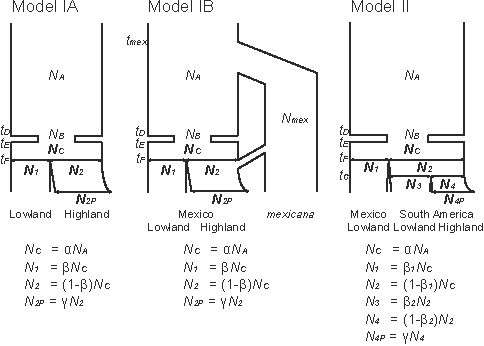
\includegraphics[width=0.5\textwidth]{fig/Fig3}
   \renewcommand{\baselinestretch}{0.9}
   \vspace{-3mm}
   \caption{Three demographic models of maize low- and highland populations.  Parameters provided in bold were estimated in this study.  See text for details.
   }
\vspace{-6mm}
    \label{model}
  \end{center}
\end{figure}
%%%%%%%%%%%%%%%%%%%%%%%%%%%%%%%%%%%%%%%%%% FIGURE

\subsubsection{Model I}
This model is applied to the Mexico and SA populations.
We assume the ancestral diploid population representing \emph{parviglumis} follows a standard Wright-Fisher model with constant size.  The size of the ancestral population is denoted by $N_A$.
At $t_D$ generations ago, the bottleneck event begins at domestication, and at $t_E$ generations ago, the bottleneck ends.  The population size and duration of bottleneck are denoted by $N_B$ and $t_B=t_D-t_E$, respectively.  The population size recovers to $N_C=\alpha N_A$ in the lowlands.  
Then, the highland population is differentiated from the lowland population at $t_F$ generations ago.  The size of the low- and highland populations at time $t_F$ is determined by a parameter, $\beta$ such that the population is divided by $\beta N_C$ and $(1-\beta)N_C$.  
We assume that the population size in the lowlands is constant but that the highland population experiences exponential expansion after divergence: its current population size is $\gamma$ times larger than that at $t_F$.  \\

\subsubsection{Model II}
We expand Model I for the Mexico populations.  We incorporate admixture from \emph{mexicana} to the highland Mexican maize population.  The time of differentiation between \emph{parviglumis} and \emph{mexicana} occurs at $t_{mex}$ generations ago.  The size of the \emph{mexicana} population is denoted by $N_{mex}$ and this size is assumed to be constant.  At $t_F$ generations ago, the Mexico highland population is derived from the Mexico lowland population and admixture with \emph{mexicana}.  The proportion of admixture with \emph{mexicana} is denoted by $P_{mex}$.  \\

\subsubsection{Model III}
The final model is for the Mexico lowland, SA lowland and SA highland populations.  This model was used for simulating SNPs with ascertainment bias (see below).  At time $t_F$, the Mexico and SA lowland populations are differentiated, and the sizes of populations after splitting are determined by $\beta_1$.  At time $t_G$, SA lowland and highland populations are differentiated, and the sizes of populations at this time are determined by $\beta_2$.  As in Model I, the SA highland population is assumed to experience population growth with the parameter, $\gamma$.\\


%%%%%%%%%%%%%%%%%%%%%%%%%%%%%%%%%%%%%%%%%% FIGURE
\begin{figure}[tb]   
  \begin{center}
   \vspace{-0mm}
   %\includegraphics[width=0.23\textwidth]{figs/model}
   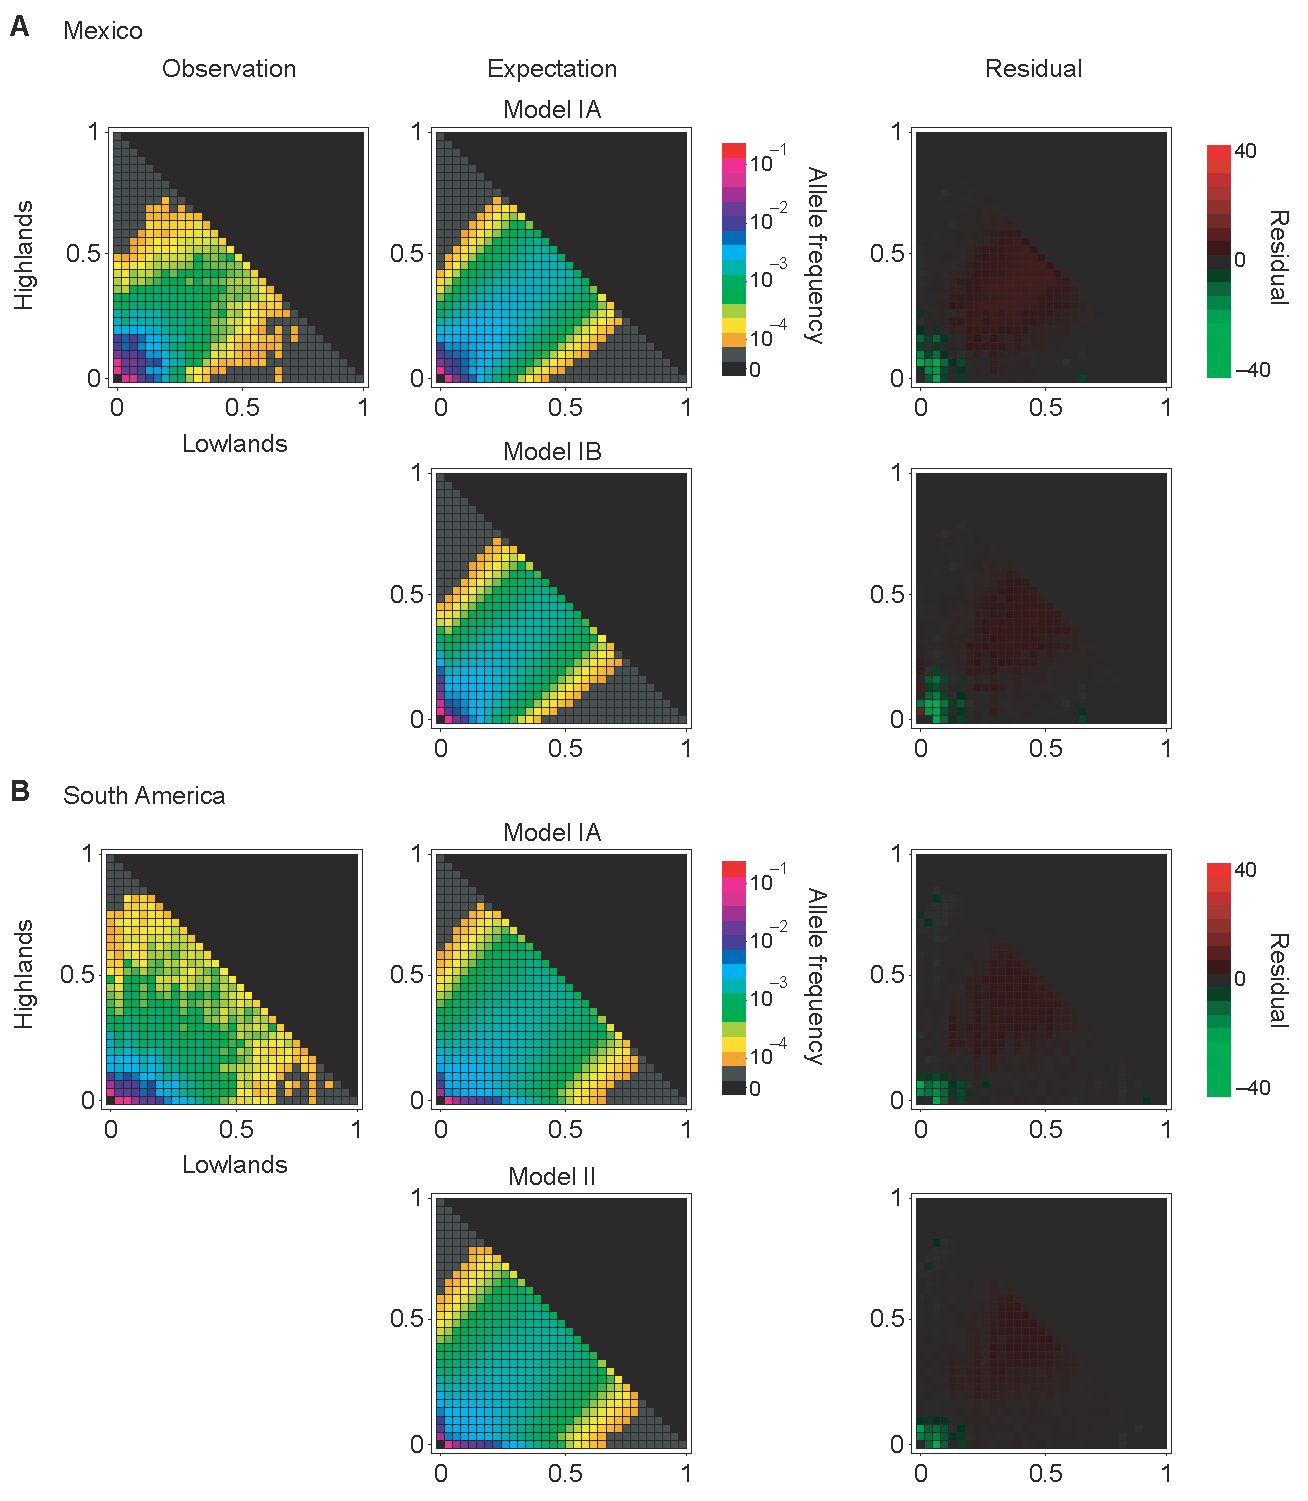
\includegraphics[width=0.5\textwidth]{fig/Fig4}
   \renewcommand{\baselinestretch}{0.9}
   \vspace{-3mm}
   \caption{Observed and expected joint distributions of minor allele frequencies in low- and highland populations in (A) Mexico and (B) South America. }
\vspace{-6mm}
    \label{JFD}
  \end{center}
\end{figure}
%%%%%%%%%%%%%%%%%%%%%%%%%%%%%%%%%%%%%%%%%% FIGURE

Estimates of a number of our model parameters were available from previous work.    
$N_A$ was determined using estimates of the composite parameter $4N_A\mu$ and a separate estimate of mutation rate, $\mu$, per site per generation.  $4N_A\mu$ was estimated in \emph{parviglumis} to be $\sim$0.018  \cite[]{Eyre-Walker_1998_9539756,Tenaillon_2001_11470895,Tenaillon_2004_15014173,Wright_2005_15919994,Ross-Ibarra_2009_19153259}.  
The mutation rate in maize has been estimated to be $2.9\sim 3.3\times 10^{-8}$, so we assume $\mu=3\times 10^{-8}$ \cite[]{Clark_2005_16079248}.  
Thus, $N_A$ was set to $0.018/4/(3\times 10^{-8}) = 150,000$.
The severity of the domestication bottleneck is represented by $k=N_B/t_B$ \cite[]{Eyre-Walker_1998_9539756,Wright_2005_15919994}, and following \cite{Wright_2005_15919994} we assumed $k=2.45$ and $t_B=1,000$ generations.  
Taking into account archaeological evidence \cite[]{Piperno_2009_19307570}, we assume $t_D=9,000$ and $t_E=8,000$.  
We further assumed $t_F=6,000$ for Mexican populations in Models I and II \cite[]{Piperno_2006_69}, $t_F=4,000$ for South American populations in Model I \cite[]{Perry_2006_16511492}, and $t_{mex}=60,000$, $N_{mex}=160,000$ \cite[]{Ross-Ibarra_2009_19153259}, and $P_{mex}=0.2$ \cite[]{vanHeerwaarden_2011_21189301} for Model II. 
For both Models I and II, we inferred three parameters ($\alpha$, $\beta$ and $\gamma$), and, for Model III, we fixed $t_F=6,000$ and $t_G=4,000$ \cite[]{Piperno_2006_69,Perry_2006_16511492} and estimated the remaining four parameters ($\alpha$, $\beta_1$, $\beta_2$ and $\gamma$).

\subsection*{Differentiation between low- and highland populations}
We used our inferred demographic model to generate a null distribution of $F_{ST}$ via simulation using the software {\sf ms} \cite[]{Hudson_2002_11847089}.   
The command line options for {\sf ms} are provided in supp Table 2.  
For each combination of sample sizes in low- and highland populations, we generated $10^7$ $F_{ST}$ values and used these as a null distribution in order to evaluate our GBS data.   We calculated $F_{ST}$ values for all SNPs that had $\geq10$ individuals with no missing data in all four populations and showed no departure from HWE at the 0.5\% level. 

Generating the null distribution of differentiation ufor the MaizeSNP50 data requires accounting for ascertainment bias. Evaluation of genetic clustering in our data (not shown) coincides with previous work \cite[]{Hufford_2012_22660546} in suggesting that the two lines most important in the ascertainment panel are most closely related to Mexican lowland maize.  
We thus added two additional individuals to the Mexican lowland population and generated our null distribution using only SNPs where the two individuals had different alleles. 
We used all SNPs where $\geq10$ individuals had no missing data in all four populations and where there was no departure from HWE at the 5\% level. i

\subsection*{Haplotype scoring test}
We performed a \underline{p}airwise \underline{h}aplotype \underline{s}coring (PHS) test to detect further evidence of selection, following \cite{Toomajian_2006_16623598}.  
To conduct this test, we first imputed and phased the combined SNP data (both GBS and MaizeSNP50) using the {\sf fastphase} software ver. 1.4.0 \cite[]{Scheet_2006_16532393}.  
As a reference for phasing, we used data (excluding heterozygous SNPs) from an Americas-wide sample of 23 partially inbred landraces that were included in the Hapmap v2 data set  \cite[]{Hufford_2012_22660546}.  
%should really cite Chia here instead of Hufford. 
{\sf fastphase} was run with default parameter settings.  PHS was calculated for an allele \emph{A} at position $x$ by

\begin{equation}
  \label{phs-1}
  \begin{array}{l}
  \displaystyle{
PHS_{x_A} = \sum^{p-1}_{i=1}\sum^{p}_{j=i+1}Z_{ijx}  / \Bigl( \begin{array}{c} p \\ 2 \\ \end{array} \Bigr) 
- \sum^{n-1}_{i=1}\sum^{n}_{j=i+1}Z_{ijx}  / \Bigl( \begin{array}{c} n \\ 2 \\ \end{array} \Bigr) 
  }
  \end {array} 
  \textrm{,}
\end{equation}

\noindent where $n$ is sample size of haploids, $p$  is the number of haploids carrying the allele $A$ at position $x$, and

\begin{equation}
  \label{phs-2}
  \begin{array}{l}
  \displaystyle{
Z_{ijx} = \frac{ d_{ijx} - \bar{d_{ij}} }{ \sigma_{ij} }
  }
  \end {array} 
  \textrm{,}
\end{equation}

\noindent where $d_{ijx}$ is the genetic distance over which individuals $i$ and $j$ are identical surrounding position $x$, $\bar{d_{ij}}$ is the genome-wide mean of distances over which individuals are identical, and $\sigma_{ij}$ is the standard deviation of the distribution of distances.  
The \emph{P}-value for an allele $A$ with frequency $p$ at position $x$ was calculated such that Pr($PHA_{xA}\leq PHA_{null|p}$), where $PHA_{null|p}$ are the PHS values for all alleles with frequency $p$ across the genome. 
%is $PHA_{p}$ a mean? The previous sentence needs to be clarified.

Genetic distances were obtained from the IBM mapping population \cite[]{Ganal_2011_22174790}.  
While genetic positions were initially only available for the MaizeSNP50 data set, we fit genetic (cM) and physical (bp) distances to a tenth degree polynomial curve, and calculated cM for all SNPs. 
%please provide the genetic map positions for all SNPs. probably not needed in the paper, but I would like this data.
 
%^JRI EDITS STOP HERE^

%%%%%%%%%%%%%%%%%%%%%%%%%%%%%%%%%%%%%%%%%% FIGURE
\begin{figure}[tb]   
  \begin{center}
   \vspace{-0mm}
   %\includegraphics[width=0.23\textwidth]{figs/model}
   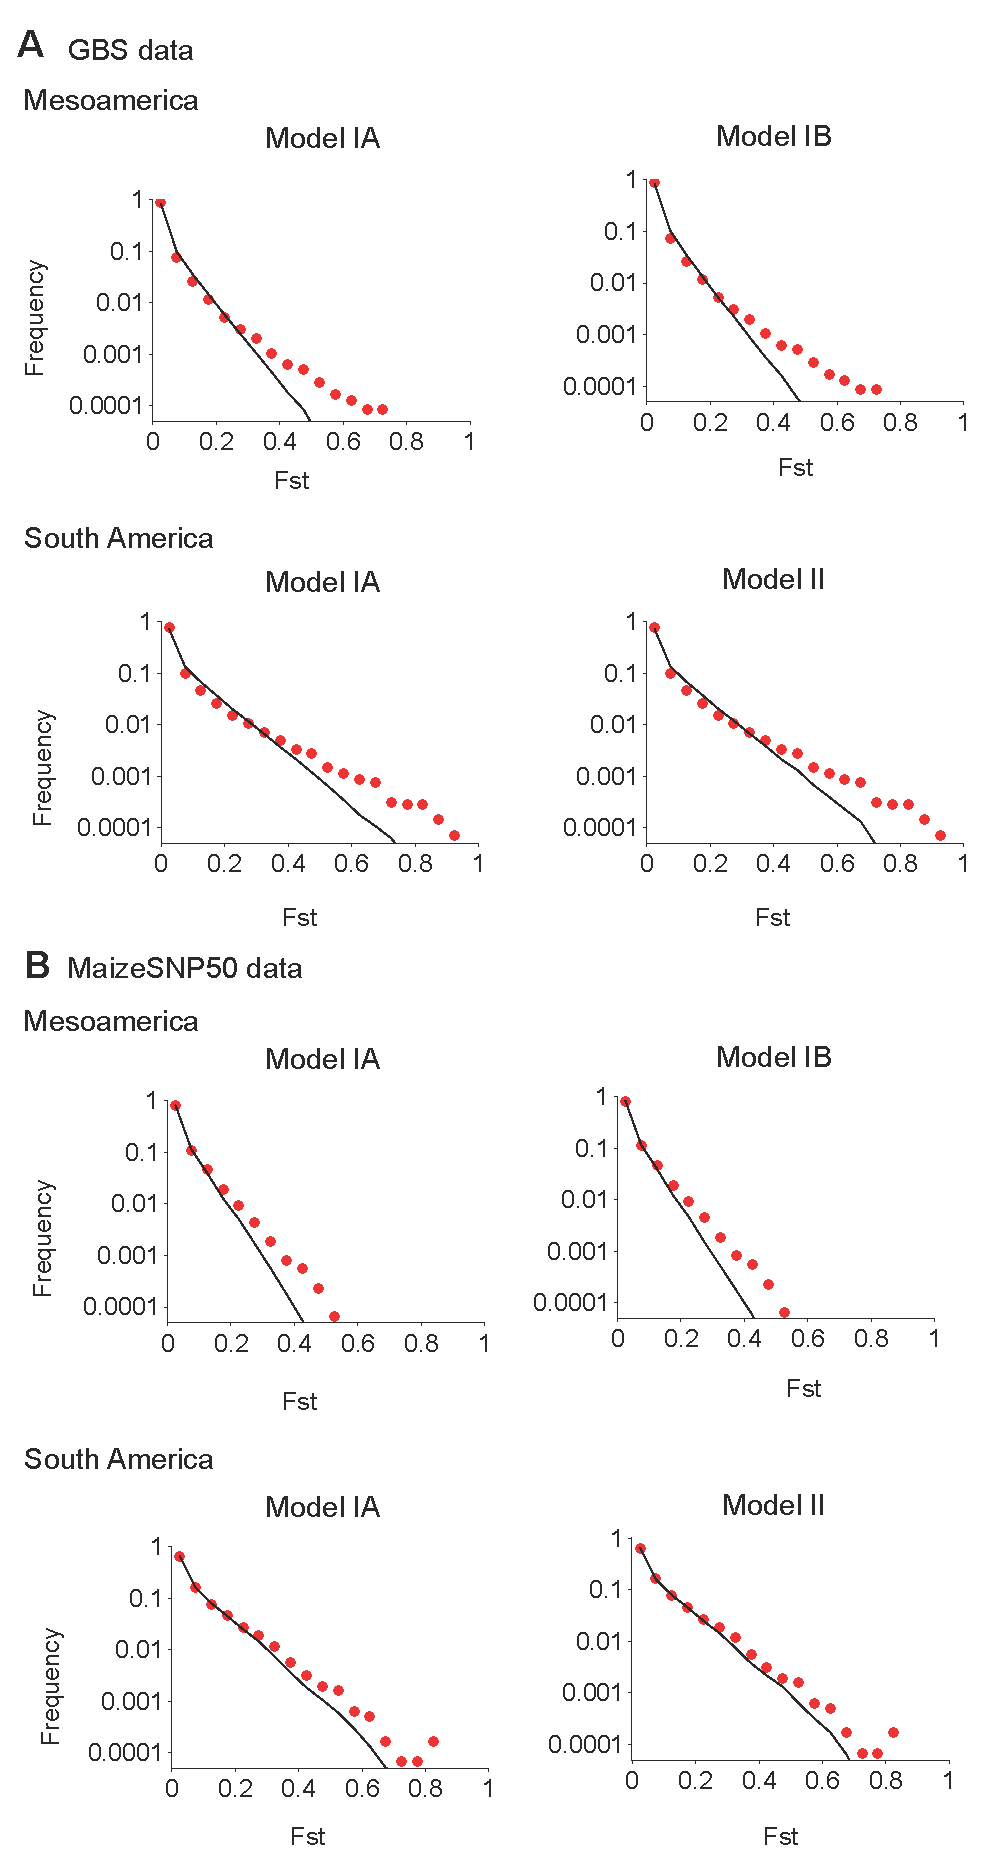
\includegraphics[width=0.45\textwidth]{fig/Fig5}
   \renewcommand{\baselinestretch}{0.9}
   \vspace{-3mm}
   \caption{Observed and expected distributions of $F_{ST}$ values in GBS (A) and MaizeSNP50 data (B).  The \emph{x}-axes represent $F_{ST}$ values.  The \emph{y}-axes represent the frequency of SNPs with $F_{ST}$ values within a bin of 0.05 size.  Red dots and solid lines indicate observed and expected distributions. 
   }
\vspace{-6mm}
    \label{FstDist}
  \end{center}
\end{figure}
%%%%%%%%%%%%%%%%%%%%%%%%%%%%%%%%%%%%%%%%%% FIGURE


%%%% PLR:
\subsection*{Migration and new mutation of adaptive alleles}

We suggest below that many of these high-$F_{ST}$ alleles are locally adaptive,
and the degree of coincidence between highland regions informs us about 
whether these adaptations occurred indpendently (in parallel), or if alleles transited between the two.
To see if the abundance and degree of coincidence is consistent with what is known about the population history of maize,
we evaluated the rate at which we expect an allele that provides a selective advantage at higher altitude
to arise by new mutation in a highland region ($\mutrate$),
and the rate at which such an allele already present in the Mexican highlands
would transit the intervening lowlands and fix in the Andean highlands ($\migrate$),
in both cases assuming it is slightly deleterious at lower altitude.
These numbers depend most strongly on the population density, 
the selection coefficient,
and the rate at which seed is transported long distances and replanted.
We evaluated these rates using new and existing theory, and validated by simulation.

\plr{
A note here on why we assume it is deleterious?  
It would be possible to say convincing things about the case where it is neutral at low elevation,
but will require significant thinking (which I've begun to do\dots).
}

To calculate the rate at which new mutations appear and fix in the highland population, $\mutrate$,
we simply used the total population size of the highlands
multiplied by the mutation rate per generation
and by the chance that a single such mutation successfully fixes
(i.e.\ is not lost to drift).
The latter probability, that a single new mutant allele providing benefit $s_b$ to heterozygotes at high elevation
will increase in frequency and fix in the high elevation patch,
is approximately $2s_b$ divided by the variance in offspring number \citep{jagers1975branching}.
This is not quite right, since such a mutation could occur at low elevation,
where it is deleterious,
and its offspring could then migrate to high elevation and fix there.
Similarly, if we use the selection coefficient for high elevation,
this ignores the fact that some of the seeds from the high-elevation plants may be grown at low elevation,
reducing the chance of fixation of an allele that appears at high elevation.
This scenario has been well-studied in theoretical models by \citet{polk} and \citet{barton1987establishment},
% missing reference for Polk.
but it is not immediately obvious how well their approximations apply to maize,
as it grows across an altitudinal gradient (rather than an abrupt transition) and has high variance in number of offspring.
Therefore, we used the following more detailed demographic model (following \citet{vanHeerwaarden2010}) 
%cite van Heerwaarden  2010 Heredity
to numerically calculate the chance of fixation of a beneficial allele
as a function of the location it first appears.
We found that the simple approximation is quite good,
although the demographic model was necessary to find the variance in offspring number,
as well as the migration rate, which we will need later.

TODO: describe demographic model in words.  (including migration which we need later.)
Reference math and more detail in appendix.

\plr{could alternatively: (a) describe the math; or (b) cut this down further.}

Concretely, the probability that a new mutation destined for fixation
will arise in a patch of high-elevation habitat of area $A$ in a given generation
is a function of the density of maize per unit area $\rho$,
the selective benefit $s_b$ it provides,
the mutation rate $\mu$,
and the variance in offspring number $\xi^2$.
In terms of these parameters, the rate of appearance is
\begin{align} \label{eqn:mutrate}
  \mutrate = \frac{2 \mu \rho A s_b}{\xi^2} .
\end{align}

A corresponding expression for the chance that an allele moves from one highland population to another is harder to intuit,
and is addressed in more depth in \citep{ralphcoop2013patches}.
If an allele is beneficial at high elevation, and fixed in the Mexican highlands,
but deleterious at low elevations,
then it will be present at low frequency in nearby lowland populations,
maintained at migration-selection balance \citep{slatkin1973geneflow}.
(Here ``migration'' is mediated by farmer exchange of seed stocks.)
This equilibrium frequency decays exponentially with distance,
so that the highland allele is present at distance $R$ from the highlands at frequency $C \exp(- R \sqrt{2s_m} / \sigma)$,
where $s_m$ is the deleterious selection coefficient for the allele in low elevation,
$\sigma$ is the mean dispersal distance (mean distance between parent and offspring),
and $C$ is a constant depending on geography ($C\approx 1/2$ is close).
Multiplying this frequency by a population size gets the predicted number of individuals carrying the allele in that population,
which at large distances can be less than 1;
this is possible because this is the average density of selected alleles across a large number of generations.
Therefore, in a lowland population of size $N$ at distance $R$ from the highlands,
$(N/2)  \exp(- R \sqrt{2s_m} / \sigma)$ is equal to the probability that there are any highland alleles present,
multiplied by the expected number of these, given that there are some present.
Since the latter is at least 1,
the chance there are any present in a given generation is no more than $(N/2) \exp(- R \sqrt{2s_m} / \sigma)$,
and so this puts an upper bound on $\migrate$.
Therefore, we would need to wait around $\Tmig = (2/N)\exp(R \sqrt{2s_m} / \sigma)$ generations 
for a rare such excursion to occur.
Concretely, we can use that
\begin{align}
  \migrate \le (N/2)  \exp(- R \sqrt{2s_m} / \sigma) ,
\end{align}
with $N$ the total size of the unadapted highland population,
and $R$ the distance from the adapted to the yet-undapted highland populations.
Another factor this omits is the probability that such an allele fixes;
however, since such alleles arrive by migration, which are planted out into a field,
it is not too bad, and conservative, to neglect the factor of $2s_b/\xi^2$,
if we count $N$ as the number of \emph{parent} plants used to replant the region each year.

To obtain specific predictions,
we then computed $\mutrate$ and $\migrate$ at various paramter values.
We also checked these with simulations and more detailed computations,
described in the Appendix.
\plr{I am flexible about what goes in that appendix\dots}
